\documentclass{article}

\author{Philip Hale}
\title{Natural Language Processing: Assessment 2}

\usepackage{graphicx}
\usepackage{epstopdf}
\usepackage{minted}


\begin{document}

\maketitle

\section{Task 1: Grammar development – 50\%}

\begin{figure}
  \centering
  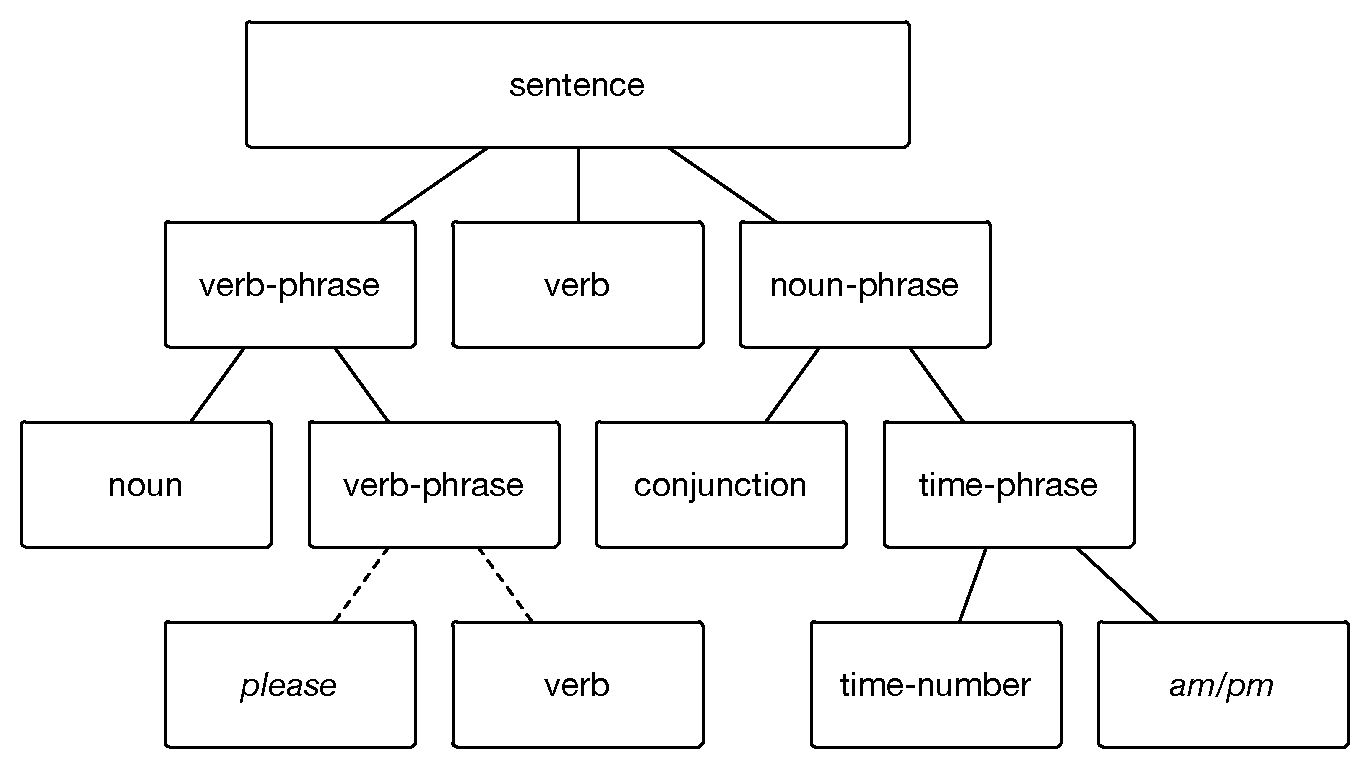
\includegraphics[width=\textwidth]{dcg_grammar.eps}
  \caption{DCG Grammar}
  \label{fig:dcg_grammar}
\end{figure}

See Figure~\ref{fig:dcg_grammar} for a graphical representation of the following
DCG grammar:

\begin{minted}[fontsize=\footnotesize]{prolog}
sentence           --> verb_phrase, verb, noun_phrase.
verb_phrase        --> noun, verb_please_phrase.
verb_phrase        --> noun, verb.
verb_please_phrase --> [please], verb.
noun_phrase        --> conjunction, time_phrase.
conjunction        --> [before, after].
time_phrase        --> time_number, [am, pm].
time_number        --> [one, two, three, four, five, six, seven, eight, nine].
time_number        --> [one, two, three, four, five, six, seven, eight, nine],
                       [ten, twenty, thirty, fourty, fifty].
\end{minted}

\section{Task 2: Semantic interpretation – 30\%}

\begin{figure}
  \centering
  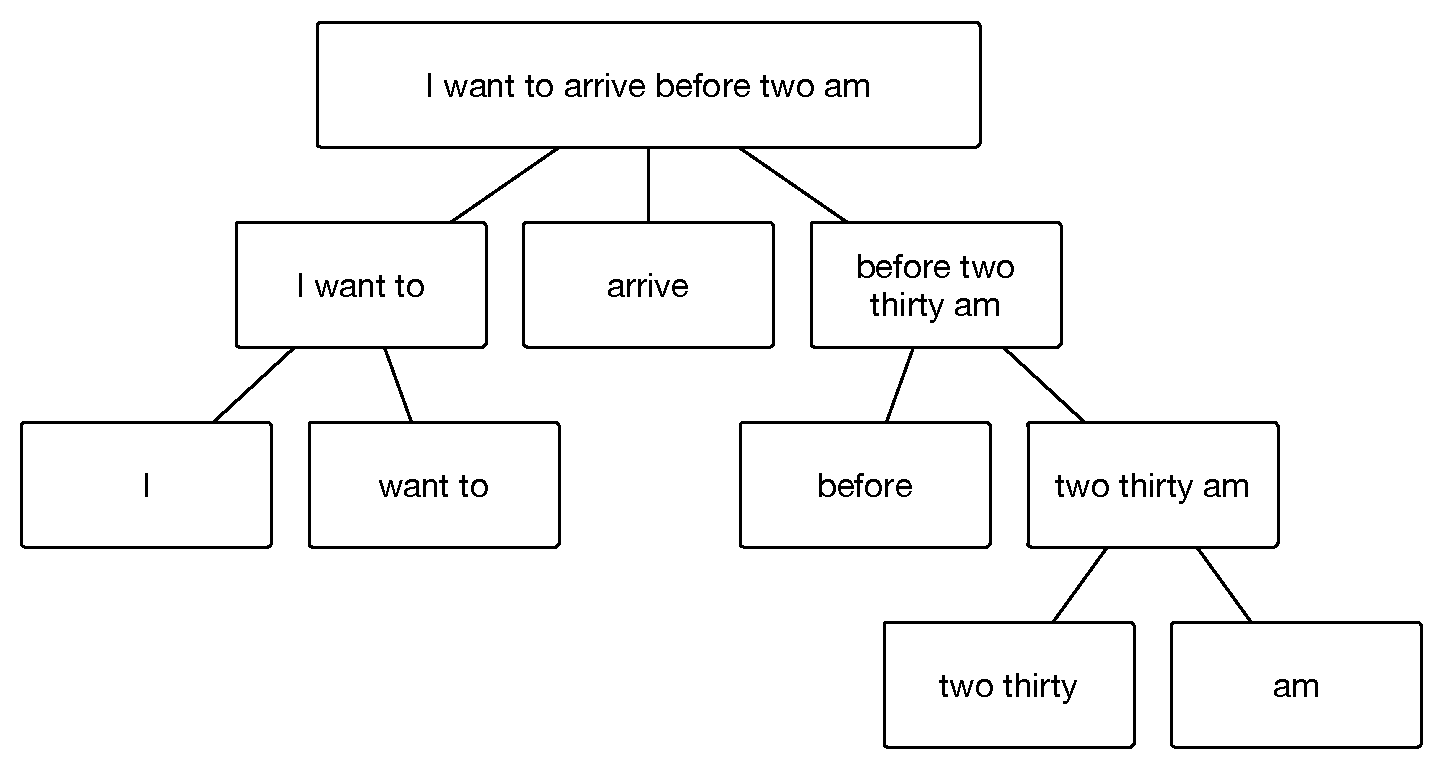
\includegraphics[width=\textwidth]{semantic_interpretation.eps}
  \caption{Parse Tree}
  \label{fig:semantic_interpretation}
\end{figure}

See Figure~\ref{fig:semantic_interpretation} for a parse tree of the sentence:
"I want to arrive before two-thirty am".

\subsection{Semantic Attachment}

{\small \verb!noun.sem + verb_phrase.sem + verb.sem + conjunction.sem + time_phrase.sem!}

\section{Task 3: Discussion of the approach – 20\%}

Statistical Information Retrieval would be an example of one such alternative
approach to semantic interpretation. It would likely be challenging in our
imaginary travel application, since the document sizes are very small. That
said, in the specific domain of air-travel, the high-volume of potential data to
learn form and relatively limited ambiguity in word phrases would make
statistical approaches quite successful. The simple nature of our task probably
does not warrant the complexity of a corpus-based model of semantics, but this
might not be the case if the set of considered sentences were broadened to
include more diverse semantics.

\end{document}

